\documentclass[12pt]{beamer}
\usepackage[utf8]{inputenc} % style d'écriture
\usepackage[T1]{fontenc}      % package
\usepackage[french]{babel}  % package pour langue française
\usepackage{graphicx}
\usepackage{subcaption}
\usepackage{url}
\usepackage{color}
\usepackage{geometry}
\usepackage{amssymb}
\usepackage{multirow, makecell}
\usepackage{listings}

% William PENSEC, étudiant en Master 2 LSE 2020/2021

\usetheme[secheader]{Madrid}
\beamertemplatenavigationsymbolsempty
\setbeamertemplate{frametitle continuation}{}

\lstset{
  aboveskip=5mm,
  belowskip=-2mm,
  basicstyle=\footnotesize,
  breakatwhitespace=false,
  breaklines=true,
  captionpos=b,
  commentstyle=\color{red},
  deletekeywords={...},
  escapeinside={\%*}{*)},
  extendedchars=true,
  framexleftmargin=16pt,
  framextopmargin=3pt,
  framexbottommargin=6pt,
  frame=tb,
  keepspaces=true,
  keywordstyle=\color{blue},
  language=C++,
  literate=
  {²}{{\textsuperscript{2}}}1
  {⁴}{{\textsuperscript{4}}}1
  {⁶}{{\textsuperscript{6}}}1
  {⁸}{{\textsuperscript{8}}}1
  {€}{{\euro{}}}1
  {é}{{\'e}}1
  {è}{{\`{e}}}1
  {ê}{{\^{e}}}1
  {ë}{{\"{e}}}1
  {É}{{\'{E}}}1
  {Ê}{{\^{E}}}1
  {û}{{\^{u}}}1
  {ù}{{\`{u}}}1
  {â}{{\^{a}}}1
  {à}{{\`{a}}}1
  {á}{{\'{a}}}1
  {ã}{{\~{a}}}1
  {Á}{{\'{A}}}1
  {Â}{{\^{A}}}1
  {Ã}{{\~{A}}}1
  {ç}{{\c{c}}}1
  {Ç}{{\c{C}}}1
  {õ}{{\~{o}}}1
  {ó}{{\'{o}}}1
  {ô}{{\^{o}}}1
  {Õ}{{\~{O}}}1
  {Ó}{{\'{O}}}1
  {Ô}{{\^{O}}}1
  {î}{{\^{i}}}1
  {Î}{{\^{I}}}1
  {í}{{\'{i}}}1
  {Í}{{\~{Í}}}1,
  morekeywords={*,...},
  numbers=left,
  numbersep=10pt,
  numberstyle=\tiny\color{black},
  rulecolor=\color{black},
  showspaces=false,
  showstringspaces=false,
  showtabs=false,
  stepnumber=1,
  stringstyle=\color{gray},
  tabsize=4,
  title=\lstname,
}

\title[Compte rendu de stage n\textsuperscript{o}13]{Coopération de drones dans un système hétérogène}
\subtitle{Compte rendu de stage n\textsuperscript{o}13}
\author{William \textsc{Pensec}}
%\author{William \textsc{Pensec}}
%\author{William \textsc{Pensec}}
\institute[Lab-STICC]{Lab-Sticc}
\date{\today}

\AtBeginSection[]
{
\begin{frame}<beamer>{Sommaire}
\tableofcontents[currentsection,currentsubsection, 
    hideothersubsections, 
    sectionstyle=show/shaded,
]
\end{frame}
}

\begin{document}
	% ---------------------------------------------------------------- %
	\begin{frame}
		\begin{titlepage}
			\begin{figure}[H]
				\centering
				
\includegraphics[scale=.15]{labsticc.png}
				\hspace{3cm}
				
\includegraphics[scale=.3]{ubo.png}
			\end{figure}
		\end{titlepage}
	\end{frame}
	
	% ---------------------------------------------------------------- %
	\section*{Sommaire}
	\begin{frame}
		\frametitle{Sommaire}
		\begin{center}
			\tableofcontents
		\end{center}
	\end{frame}
	%
	% ---------------------------------------------------------------- %
	\section{Mouvements d'un point A à un point B}
	\begin{frame}[allowframebreaks]
    	    % Finir mouvements du drone d'un point A vers point B
    	    % Prendre des photos (beaucoup) DONE
    	    % Voir si zoom possible avec la caméra NON DONE
    	    % Préparation article
    	    % Préparation rapport de stage
    	    % Tester scenario/scenarii mouvement de drone
    	    % Faire un dataset des anomalies (entre 4 et 10)
    	    %   - pas assez de bille dans le tube = recette non exécutée
    	    %   - pas de tube sur la plate-forme
    	    %   - pas de bouchon sur la plate-forme
    	    %   - levier qui reste bloqué à un endroit
    	    %   - convoyeur qui se bloque
    	    % Utiliser LeNET-5 pour réseau de neurones
    	    % Magnetometre : X (Est / Ouest) , Y (Nord / Sud), Z (Profondeur)
    	    
    	     \begin{block}{Utilisation du magnétomètre}
    	        \begin{itemize}
    	            \setbeamertemplate{itemize item}[triangle]
    	            \item Fonction disponible pour récupérer la valeur en X, Y, Z
    	            \item Documentation très incomplète
    	            \item Nécessité de calibrer le drone pour bien utiliser le capteur (impossible dans la pièce)
    	            \item Valeurs différentes selon les endroits dans la pièce
    	        \end{itemize}
    	    \end{block}
    	    
    	    \begin{figure}
			    \centering
			    \includegraphics[width=0.65\linewidth]{magDoc.png}
			\end{figure}
    	    
    	    \begin{figure}
			    \centering
			    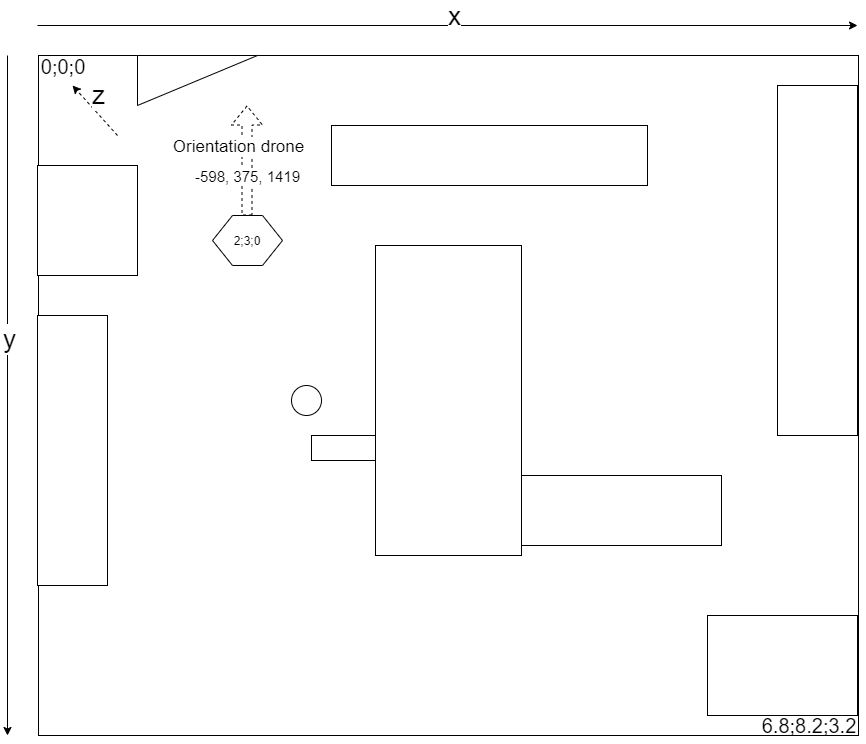
\includegraphics[width=0.8\textwidth]{calibrationMagnetoNord.png}
			\end{figure}
			
    	    \begin{figure}
			    \centering
			    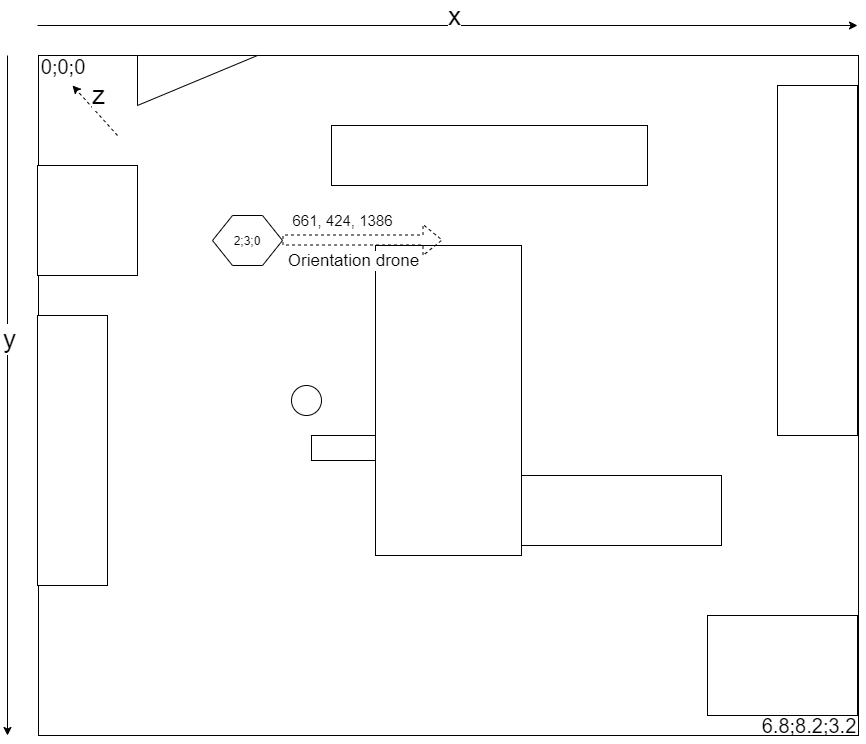
\includegraphics[width=0.8\textwidth]{calibrationMagnetoEst.png}
			\end{figure}
			
    	    \begin{figure}
			    \centering
			    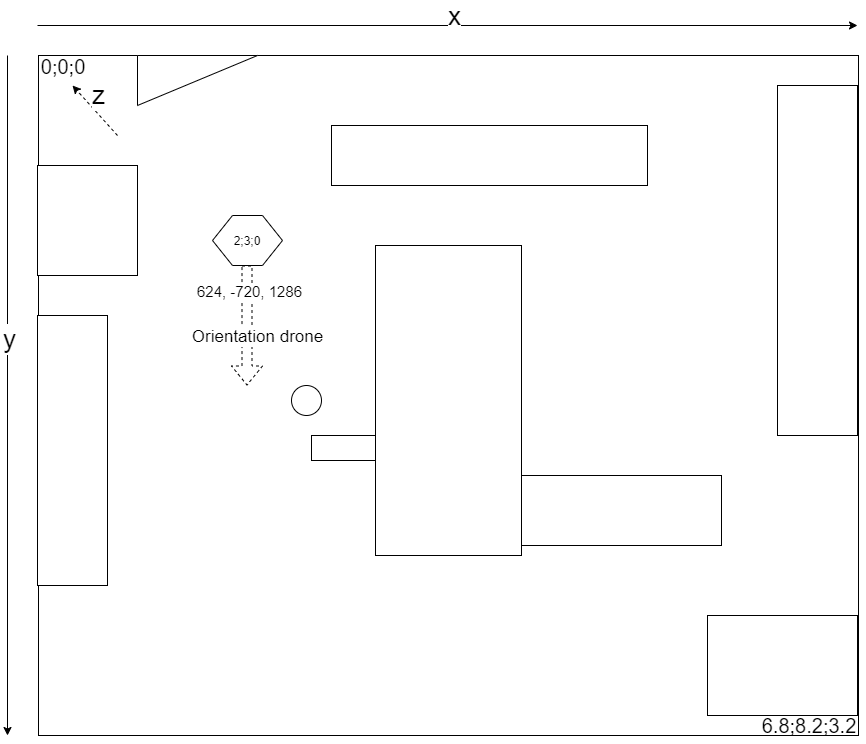
\includegraphics[width=0.8\textwidth]{calibrationMagnetoSud.png}
			\end{figure}
			
    	    \begin{figure}
			    \centering
			    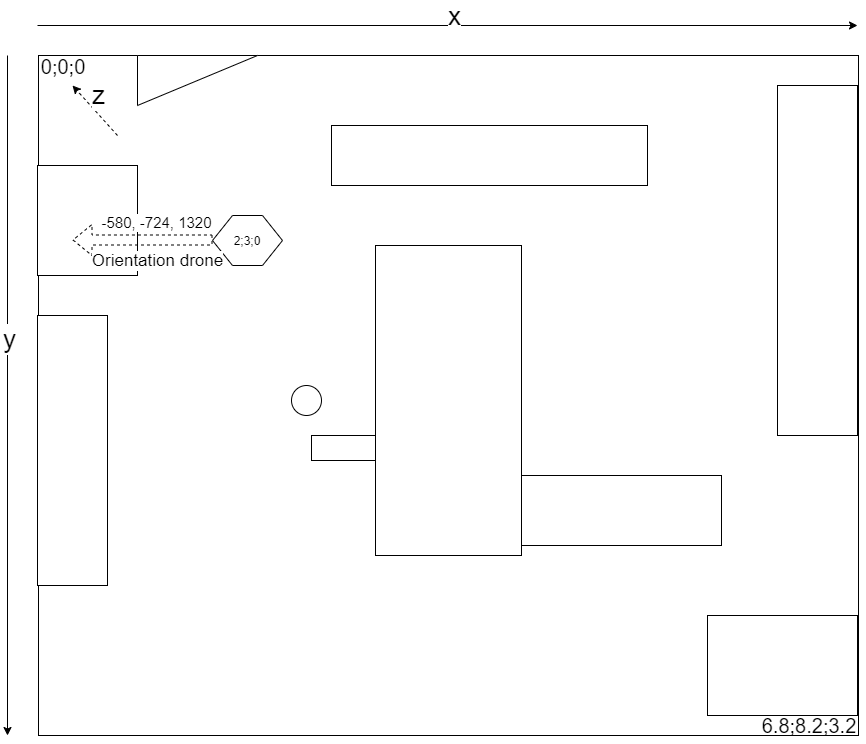
\includegraphics[width=0.8\textwidth]{calibrationMagnetoOuest.png}
			\end{figure}
	\end{frame}
	%
	% ---------------------------------------------------------------- %
	\section{Caméra du raspberry pi}
	\subsection{Prise de 1500 photos}
	\begin{frame}[allowframebreaks]
	    \begin{figure}
		    \centering
		    \includegraphics[width=0.8\textwidth]{imageJour.png}
		    \caption*{Image avec lumière allumée}
		\end{figure}
		\begin{figure}
		    \centering
		    \includegraphics[width=0.8\textwidth]{imageNuit.png}
		    \caption*{Image avec lumière éteinte}
		\end{figure}
		
	    \begin{figure}
		    \centering
		    \includegraphics[width=0.8\textwidth]{imageGauche.png}
		    \caption*{Image à la gauche du point visé}
		\end{figure}
		\begin{figure}
		    \centering
		    \includegraphics[width=0.8\textwidth]{imageMilieu.png}
		    \caption*{Image au milieu du point visé}
		\end{figure}
		\begin{figure}
		    \centering
		    \includegraphics[width=0.8\textwidth]{imageDessus.png}
		    \caption*{Image au dessus du point visé}
		\end{figure}
	\end{frame}
	%
	% ----------------------------------- %
	\subsection{Divers}
	\begin{frame}[allowframebreaks]
	    \begin{block}{}
	        \begin{itemize}
	            \setbeamertemplate{itemize item}[triangle]
	            \item Zoom impossible 
	            \item Possibilité de rogner la photo afin de capturer seulement ce que l'on veut (diminue la définition de l'image)
	        \end{itemize}
	    \end{block}
	    
	    \begin{figure}
		    \centering
		    \includegraphics[width=0.8\textwidth]{imageFull.png}
		    \caption*{Image entière}
		\end{figure}
		
		\begin{figure}
		    \centering
		    \includegraphics[width=0.6\textwidth]{imageCroped.png}
		    \caption*{Image rognée}
		\end{figure}
	\end{frame}
	%
	% ---------------------------------------------------------------- %
	\section{Exemple d'anomalies possible à détecter}
	\begin{frame}
	    \begin{block}{}
	        \begin{itemize}
	            \setbeamertemplate{itemize item}[triangle]
	            \item Pas assez de bille dans le tube = recette mal exécutée
        	    \item Pas de tube sur la plate-forme
        	    \item Pas de bouchon sur la plate-forme
        	    \item Levier qui reste bloqué à un endroit
        	    \item Convoyeur qui s'arrête
	        \end{itemize}
	    \end{block}
	\end{frame}
	%
	%% ---------------------------------------------------------------- %
\end{document}